\chapter{Regression}
\newcommand{\linkAutoSklearnRegressor}{https://automl.github.io/auto-sklearn/master/api.html\#regression}

Within auto-sklearn, we can use the \href{\linkAutoSklearnRegressor}{'AutoSklearnRegressor'\footnote{\url{\linkAutoSklearnRegressor}}} to implement a model for a regression problem.

\section{Used Car Prices}
\newcommand{\kagglelinkusedcar}{https://www.kaggle.com/kukuroo3/used-car-price-dataset-competition-format}

% \newcommand{\kagglelinkusedcaruk}{https://www.kaggle.com/adityadesai13/used-car-dataset-ford-and-mercedes?select=vw.csv}

For our first regression problem we will build a model to predict the price for used cars.

% use the \href{\kagglelinkusedcar}{'used car price dataset'\footnote{\kagglelinkusedcar}} provided by Kaggle.

% For this dataset we used the competition version of a big data set provided on  This set is based on a big \href{\kagglelinkusedcaruk}{dataset\footnote{Used Car UK:\href{\kagglelinkusedcaruk}{\kagglelinkusedcaruk}}} of 100 000 listings on used cars in the UK. We then found and used a version that was slimmed down for competition. This dataset looked ideal for us to learn more about auto-sklearn.

\subsection{Dataset}

The dataset \href{\kagglelinkusedcar}{'used car price dataset'\footnote{\url{\kagglelinkusedcar}}} provided by Kaggle, contains 12 features which can be used to predict the sales price for used cars in the UK. Those features are:

\begin{itemize}
    \item brand: The brand of the car.
    \item model: The model within the brand.
    \item year: The year of manufacturing.
    \item transmission: The type of transmission.
    \item mileage: The total amount of mileage on the car.
    \item fuelType: The type of fuel.
    \item tax: The tax amount.
    \item mpg: The fuel consumption ($mpg$).
    \item engineSize: The engine capacity.
    \item price: The sales price of the used car.
\end{itemize}

\noindent There are 4960 observations in the training dataset. For none of the features data is missing. We also have a validation dataset with 2672 entries, which will be used to validate the performance of our model.

\subsection{Model Performance}

We visualise the dataset using 2 pairplots, a \nameref{fig:PairplotFueltype} and a \nameref{fig:PairplotBrand}. We can clearly observe a positive correlation between the year of manufacturing of the vehicle and the price. Between the milage and the price, we can see a negative correlation as expected. The correlation between the price and the engine size is also positive, and we even see that the share of petrol cars with a high mileage is significantly larger.

\begin{figure}[h!]
    \begin{center}
        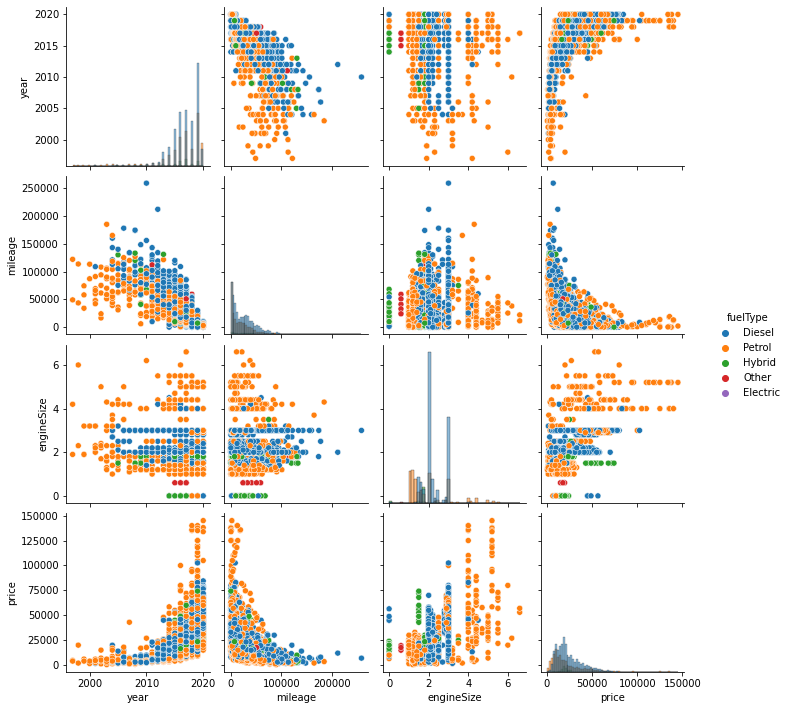
\includegraphics[width=.7\linewidth]{images/pairplot_fueltype.png}
        \caption{pairplot based on fueltype}
        \label{fig:PairplotFueltype}
    \end{center}
\end{figure}

The pairplot that is based on the brand shows clearly that the german brands are most common.

\begin{figure}[h!]
    \begin{center}
        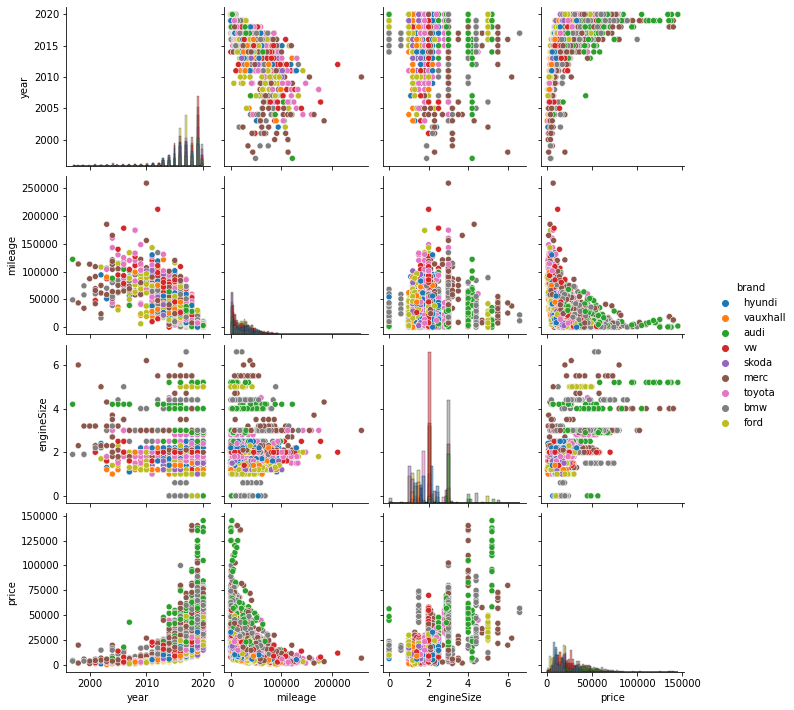
\includegraphics[width=0.7\linewidth]{images/pairplot_brand.png}
        \caption{pairplot based on brand}
        \label{fig:PairplotBrand}
    \end{center}
\end{figure}

After fitting and training the data, these are the results we got for the training, testing and validation datasets. The $r^2$-score is extremely good and almost perfect.

\begin{table}[h!]
    \begin{center}
        \caption{Table with training results.}
        \label{tab:training results}
        \begin{tabular}{l|r|r|r} % <-- Changed to S here.
            \textbf{function} & \textbf{Training data} & \textbf{Test data} & \textbf{Validation data}\\
            \hline
            mean squared error & 59050.4794 & 293230.5317 & 585230.4846\\
            mean absolute error & 26.3980 & 55.7094 & 59.8129\\
            r2 & 0.9998 & 0.9989 & 0.9979\\
        \end{tabular}
    \end{center}
\end{table}

\subsection{Model Comparision}
\newcommand{\linkUsedCarAkarshsinghh}{https://www.kaggle.com/akarshsinghh/car-price-prediction-score-93-random-forest}

\newcommand{\linkUsedCarCompareSelinsong}{https://www.kaggle.com/selinsong/u-car-rf-r2-score-0-94/data}
\newcommand{\linkUsedCarCompareYuyuyuyuy}{https://www.kaggle.com/yuyuyuyuy/rf-test-r2-score-0-956}
\newcommand{\linkUsedCarCompareJohyunkang}{https://www.kaggle.com/johyunkang/py-rf-test-r2-0-939}

When we compare our model with the previous submissions on Kaggle, we definetly score a better performance. Most of the submissions are using the 'RandomForestRegressor' and where some of them even dropped \href{\linkUsedCarAkarshsinghh}{the 'model' feature}, we've opt to keep this feature, and make sure our dummies from the trianing and validation dataset align corretly.

% \begin{table}[h!]
%     \begin{center}
%         \caption{Table with r2 results.}
%         \label{tab:training results}
%         \begin{tabular}{l|l} % <-- Changed to S here.
%             \textbf{data} & \textbf{R2 score} \\
%             \hline
%             Training data & 0.9997784238195022\\
%             Test data & 0.9989334899119373 \\
%             Validation data & 0.9978756073515518\\
%             Url1 & 0.94\\
%             Url2 & 0.956\\
%             Url3 & 0.939\\
%         \end{tabular}
%     \end{center}
% \end{table}

\section{Television Brand E-commerce}
This dataset is used to explore the current market share for television contructors. There are various types of screens with different operating systems offered by several manufacturers at competitive prices.

\subsection{Dataset}
\newcommand{\kagglelinktv}{https://www.kaggle.com/devsubhash/television-brands-ecommerce-dataset}

This \href{\kagglelinktv}{dataset\footnote{Television dataset:\href{\kagglelinktv}{\kagglelinktv}}} includes specifications of different televisions offered by various brands with prices and ratings. It consists of 912 samples with 7 attributes. The features are:

\begin{itemize}
    \item Brand: The manufacturer of the product.
    \item Resolution: The type of display i.e. LED, HD LED, etc.
    \item Size: The screen size in inches.
    \item Selling Price: The selling price or the discounted price of the distributer.
    \item Original Price: The original price of the product from the manufacturer.
    \item Operating system: The type of OS (like Android, Linux, etc.).
    \item Rating: Average customer ratings on a scale of 5.
\end{itemize}

\subsection{Model Performance}
With a pairplot we visualise the dataset, to get a first indication about any possible correlations. We clearly see a positive correlation between the size of the display and the selling price. Also the share the category of 'ULTRA HD LED' televisions are to be situated in a higher pricing region.
\begin{figure}
    \begin{center}
        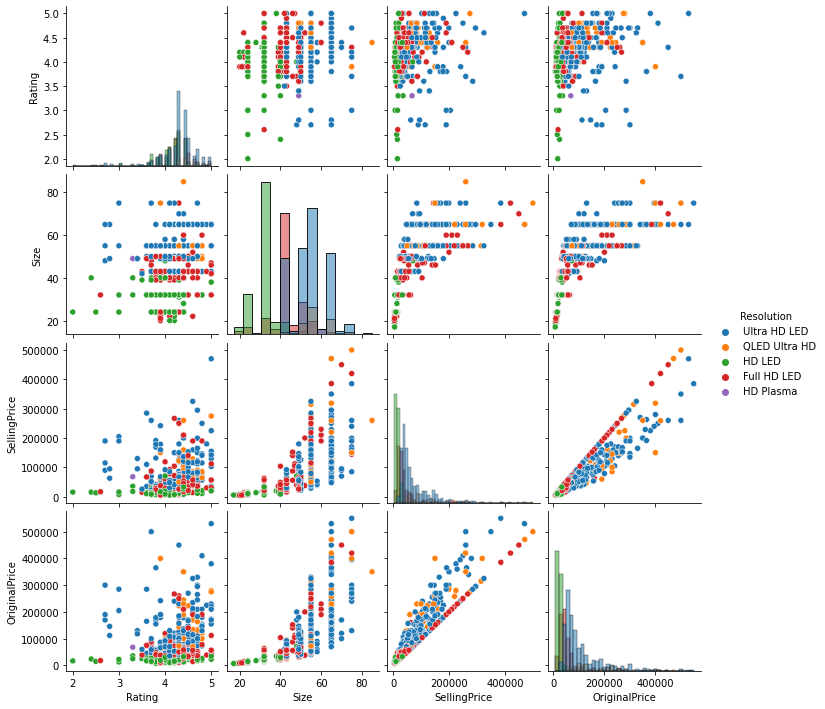
\includegraphics[width=0.7\linewidth]{images/pairplot_resolution.png}
        \caption{pairplot based on the screen resolution}
        \label{fig:PairplotResolution}
    \end{center}
\end{figure}

After fitting and training the data these are the results we got for the both the training and testing datasets.

\begin{table}[htp]
    \begin{center}
        \caption{Table with training results.}
        \label{tab:training results}
        \begin{tabular}{l|r|r} % <-- Changed to S here.
            \textbf{function} & \textbf{Training data} & \textbf{Test data} \\
            \hline
            mean squared error & 81016219.5942 & 952681194.3707 \\
            mean absolute error & 5251.9137 & 14205.9729 \\
            r2 & 0.9797 & 0.8248\\
        \end{tabular}
    \end{center}
\end{table}

We again reach a pretty good $r^2$-score for our model, both on the trianing as on the testing dataset. A feature which strongly affect the predicitons will be the original price from the manufacturer, because as we see on the \nameref{fig:PairplotResolution}, there is a very strong correlation between both.

\subsection{Model Comparision}
\newcommand{\kagglelinktvcode}{https://www.kaggle.com/devsubhash/television-brands-ecommerce-dataset/code}

On the \href{\kagglelinktvcode}{kaggle\footnote{\url{\kagglelinktvcode}}} page of this dataset we found out that there are not yet any other regression projects submitted. For this reason, we can not compare our results.